\chapter[Proton Activation \& Radioactive Decay]{Methodology: Proton Activation and Radioactive Decay}

\begin{changemargin}{1.0cm}{1.0cm}
\abstractpreamble{A computer program was developed to calculate the radioactivity of an ion irradiated target.  The choice of projectile was limited to protons, but there is the option to increase this to other light ions.  The decay equations were derived to be able to calculate the activity of isotopes within the target at time t during and after irradiation.  The simulation is split into two parts: the first with the beam on, where there will be source terms for isotopes, and the second with the beam off where there are no external source terms.  \\
\\
\acrshort{srim}, an ion transport code, was used to calculate ion trajectory data.  Iron was irradiated experimentally by 36MeV protons with the University of Birmingham cyclotron, and its activity was measured and calculated using the activity code.  Additional data where a colleague irradiated Molybdenum was also compared with that calculated by the activity code.  Initially it was developed in Fortran, but the most recent version was written in Python.\\
\\
The equations and code were then used to predict the activity of an iron sample irradiated to 100\acrshort{dpa} for a range of proton energies.  This is a reasonable damage dose that is expected in \acrshort{gen4} reactors.}
\end{changemargin}



\section{Introduction}


High flux neutron reactors are expensive to use, whereas proton accelerators capable of producing beams of adequate fluence and energy are more readily available, cheaper to buy and cheaper to run.  Ion beams, due to the Coulomb interaction, are more controllable in terms of energy, direction and fluence.  They may be concentrated on a desired target at a set fluence and energy.

Depending on the energy of the ion beam, the target material will become radioactive.  The stable nuclei are transmuted and when the resulting isotope is unstable it will decay.  An equation was derived to predict the activity of isotopes for any decay chain with source terms and branching factors included.  Two versions of a computer code were developed to compute the reaction rates and activity of the irradiated targets.



%%====================================================================================================================================================
%%
%%  Part 2: Activity Code
%%
%%====================================================================================================================================================

\section{Activation by Ion Irradiation}



The Bateman equation was derived using Laplace transforms, and this same method has been used to develop a modified equation that incorporates branching factors and production rates for each isotope in the decay chain, as illustrated by figure \ref{fig:decaytree}.

\begin{figure}[!h]
	\centering
	\begin{tikzpicture}[node distance=2cm]
	% Row 1
	\node (parent) [startstop] {Parent Isotope};
	\node (parent_source) [process, left of=parent, xshift=-4cm] {Parent Source};
	% Row 2
	\node (parent_branch) [decision, below of=parent] {Branching};
	% Row 3
	\node (daughter_1a) [process, below of=parent_branch, xshift=-2.5cm] {Daughter 1 (Branch A)};
	\node (daughter_1a_src) [process, left of=daughter_1a, xshift=-2.5cm] {External Source};
	\node (daughter_1b) [process, below of=parent_branch, xshift=2.5cm] {Daughter 1 (Branch B)};
	\node (daughter_1b_src) [process, right of=daughter_1b, xshift=2.5cm] {External Source};
	% Row 4
	\node (daughter_1a_branch) [decision, below of=daughter_1a, xshift=0.5cm] {Branching};
	% Row 5
	\node (daughter_2a) [process, below of=daughter_1a_branch, xshift=-0.5cm] {Daughter 2 (Branch A)};
	\node (daughter_2a_src) [process, left of=daughter_2a, xshift=-2.5cm] {External Source};
	\node (daughter_2b) [process, below of=daughter_1a_branch, xshift=4.5cm] {Daughter 2 (Branch B)};
	\node (daughter_2b_src) [process, right of=daughter_2b, xshift=2.5cm] {External Source};
	
	% arrows
	\draw [thick,->] (parent_source) -- (parent);
	\draw [thick,->] (parent) -- (parent_branch);
	\draw [thick,->] (parent_branch) -- (daughter_1a);
	\draw [thick,->] (parent_branch) -- (daughter_1b);
	\draw [thick,->] (daughter_1a_src) -- (daughter_1a);
	\draw [thick,->] (daughter_1b_src) -- (daughter_1b);
	\draw [thick,->] (daughter_1a) -- (daughter_1a_branch);
	\draw [thick,->] (daughter_1a_branch) -- (daughter_2a);
	\draw [thick,->] (daughter_1a_branch) -- (daughter_2b);
	\draw [thick,->] (daughter_2a_src) -- (daughter_2a);
	\draw [thick,->] (daughter_2b_src) -- (daughter_2b);
	
	%\draw [->] (isotope1) -- (isotope2);
	%\draw [->] (isotope2) -- (stable);
	\end{tikzpicture}
	\captionsetup{font={it}}
	\caption{An example of several decay chains including branching factors and possible external source terms for each isotope on each chain.}
	\label{fig:decaytree}
\end{figure}


\subsection{Laplace Transform}
\label{section:laplaceequations}

Laplace Transforms (eq. \ref{eq:eqLaplaceTransform}) are a useful mathematical tool, and allow ordinary differential equations to be solved by simple algebraic manipulation in the s domain (appendix \ref{chapter:usefullaplacetransforms}).  Bateman took advantage of Laplace Transforms in deriving his equation, and this is the method that has been taken here as well.

\eqLaplaceTransform


\subsection{Constructing the Differential Equations}

The first step is to set up differential equations for the parent isotope, unstable daughter isotopes and stable daughter isotope.  The parent isotope has a source term, due to production, and a loss term, due to decay.  The unstable daughter isotopes have two source terms, from the production by irradiation induced transmutation and the decay of preceding isotopes in the decay chain, and a loss term, due to decay.  Finally, the stable daughter that finalizes the decay chain has two source terms (the same as the unstable daughters) but no loss term.

The variables (and vectors) used in these equations are defined as follows:
\begin{itemize}
	\item $\vec{\lambda}$  vector containing isotope decay constants $\lambda_i$
	\item $\vec{b}$  vector containing isotope to isotope branching factors $b_i$
	\item $\vec{w}$  vector containing isotope production rates $w_i$
	\item $t$  time at which activity/amount of isotope is measured
	\item $N_{i}(0)$ starting amount of the i\textsuperscript{th} isotope
	\item $N_{i}(t)$ amount of the i\textsuperscript{th} isotope at time t
	\item $N'_{i}(t)$ change in amount of the i\textsuperscript{th} isotope, with respect to time, at time t
\end{itemize}

The differential equations for the parent isotope (first isotope), unstable daughter isotopes (i\textsuperscript{th} isotopes) and stable, final, daughter isotope (zth isotope) in the time domain are as follows:

\begin{equation}
N'_{1}(t) = \omega_{1} - \lambda_{1} N_{1} (t)
\end{equation}

\begin{equation}
N'_{i}(t) = \omega_{i} + b_{i-1} \lambda_{i-1} N_{i-1} (t) - \lambda_{i} N_{i} (t)
\end{equation}

\begin{equation}
N'_{z}(t) =  \omega_{z} + b_{z-1} \lambda_{z-1} N_{z-1} (t)
\end{equation}

Applying the Laplace Transform to these three differential equations allows them to be manipulated and solved algebraically in the s-domain.

\begin{equation}
N_{1}(s) = \frac{1}{s+\lambda_{1}} N_{1}(0) + \frac{1}{s(s+\lambda_{1})} \omega_{1}
\end{equation}

\begin{equation}
N_{i}(s) = \frac{1}{s ( s+ \lambda_{i})} \left(\omega_{i} \right) + \frac{1}{s+ \lambda_{i}} \left( b_{i-1} \lambda_{i-1} N_{i-1} (s) \right) + \frac{1}{s+ \lambda_{i}} N_{i} (0)
\end{equation}

\begin{equation}
N_{z}(s) = \frac{1}{s^2} \omega_{z} + \frac{1}{s} b_{z-1} \lambda_{z-1} N_{z-1} (s) + \frac{1}{s} N_{z}(0)
\end{equation}


\subsection{Numerical Inversion of the Laplace Transform}

The Gaver-Stehfest\cite{stehfest} algorithm was developed in the 1960s and 1970s and is a method of calculating the inverse of a Laplace Transform in the real number domain.  It is an easy to implement and reasonably accurate method, although it is an approximation to the real value.  A comparison between an analytic and numeric inversion for the unstable isotope Po-218 is discussed at the end of this section (figure \ref{fig:po218decay}).

\begin{equation}
f(t) \approx f_{n}(t) = \frac{\ln(2)}{t} \sum_{k=1}^{2n} a_{k}(n)F(s) \textnormal{ where } n \ge 1, t>0
\end{equation}

\begin{equation}
s = \frac{k \ln(2)}{t}
\end{equation}

\begin{equation}
a_{k}(n) = \frac{(-1)^{(n+k)}}{n!} \sum_{j=Floor(\frac{k+1}{2})} j^{n+1} \left( \begin{matrix} n \\ j \end{matrix} \right)  \left( \begin{matrix} 2j \\ j \end{matrix} \right)  \left( \begin{matrix} j \\ k-j \end{matrix} \right)
\end{equation}

The equation for the i\textsuperscript{th} isotope may be calculated by recursively calculating the equations by numeric inversion, starting from the first (parent isotope) and inserting the result into each subsequent recursion until the i\textsuperscript{th} isotope is reached (changing the equations appropriately for the parent, unstable daughter and stable daughter isotopes).


\subsection{Analytic Solution by Partial Fraction Expansion}
\label{section:activitysolution}

The equation for the i\textsuperscript{th} isotope in the s domain can be written in full by substituting the preceding equation until the parent isotope is reached, and this full equation may be rearranged with the production amount of each isotope and starting amount of each isotope in individual terms.  Each of these terms is multiplied by a fraction that can be expanded, using partial fractions, and inverted analytically.

This is illustrated with an example unstable isotope, fourth in the decay chain (including the parent isotope) (eq. \ref{eq:example4thchainunstable}).

\begin{equation}
\begin{split}
N_{4}(s) =
\frac{1}{(s+\lambda_1)(s+\lambda_2)(s+\lambda_3)(s+\lambda_4)} b_{2} b_{3} b_{4} \lambda_1 \lambda_2 \lambda_3 N_{1}(0) \\
+ \frac{1}{(s+\lambda_2)(s+\lambda_3)(s+\lambda_4)} b_{3} b_{4} \lambda_2 \lambda_3 N_{2}(0) \\
+ \frac{1}{(s+\lambda_3)(s+\lambda_4)} b_{4} \lambda_3 N_{3}(0) \\
+ \frac{1}{(s+\lambda_4)} N_{4}(0) \\
+ \frac{1}{s(s+\lambda_1)(s+\lambda_2)(s+\lambda_3)(s+\lambda_4)} b_{2} b_{3} b_{4} \lambda_1 \lambda_2 \lambda_3 \omega_{1} \\
+ \frac{1}{s(s+\lambda_2)(s+\lambda_3)(s+\lambda_4)} b_{3} b_{4} \lambda_2 \lambda_3 \omega_{2} \\
+ \frac{1}{s(s+\lambda_3)(s+\lambda_4)} b_{4} \lambda_3 \omega_{3} \\
+ \frac{1}{s(s+\lambda_4)} \omega_{4}
\end{split}
\label{eq:example4thchainunstable}
\end{equation}

An example stable isotope, fourth (last) in the decay chain (including the parent isotope) (eq. \ref{eq:example4thchainstable}).

\begin{equation}
\begin{split}
N_{4}(s) =
\frac{1}{s(s+\lambda_1)(s+\lambda_2)(s+\lambda_3)} b_{2} b_{3} b_{4} \lambda_1 \lambda_2 \lambda_3 N_{1}(0) \\
+ \frac{1}{s(s+\lambda_2)(s+\lambda_3)} b_{3} b_{4} \lambda_2 \lambda_3 N_{2}(0) \\
+ \frac{1}{s(s+\lambda_3)} b_{4} \lambda_3 N_{3}(0) \\
+ N_{4}(0) \\
+ \frac{1}{s^2(s+\lambda_1)(s+\lambda_2)(s+\lambda_3)} b_{2} b_{3} b_{4} \lambda_1 \lambda_2 \lambda_3 \omega_{1} \\
+ \frac{1}{s^2(s+\lambda_2)(s+\lambda_3)} b_{3} b_{4} \lambda_2 \lambda_3 \omega_{2} \\
+ \frac{1}{s^2(s+\lambda_3)} b_{4} \lambda_3 \omega_{3} \\
+ \frac{1}{s^2} \omega_{4}
\end{split}
\label{eq:example4thchainstable}
\end{equation}

By using partial fraction expansion and standard Laplace Transforms, the set of equations (eqs. \ref{eq:unstable1}, \ref{eq:unstable2}, \ref{eq:unstable3}, \ref{eq:unstable4}) is used to calculate the amount of the m\textsuperscript{th} isotope in the decay chain, providing the m\textsuperscript{th} isotope is unstable.

\begin{equation}
\begin{split}
N_{m}(t; \vec{\lambda}, \vec{b}, \vec{w}, \vec{N_{0}})
= \sum_{k=1,m} r(k, m, \vec{\lambda}, \vec{b}) \left[ f(t; k,m,\vec{\lambda}) N_{0, k} + g(t;k,m,\vec{\lambda}) w_{k} \right ]
\end{split}
\label{eq:unstable1}
\end{equation}

\begin{equation}
\begin{split}
r(k,m,\vec{\lambda}, \vec{b}) =
\begin{cases}
\prod_{i=k,m-1} \left( b_{i+1} \lambda_{i} \right) , & \text{if } k < m\\
1, & \text{if }k = m
\end{cases}
\end{split}
\label{eq:unstable2}
\end{equation}

\begin{equation}
\begin{split}
f(t;k,m,\vec{\lambda})
=
(-1)^{m-k}
\sum_{i=k,m}
\left[
\frac{\exp(-\lambda_i t)}{\prod_{j=k,m;j\neq i}\left(\lambda_i-\lambda_j\right )}
\right ]
\end{split}
\label{eq:unstable3}
\end{equation}

\begin{equation}
\begin{split}
g(t;k,m,\vec{\lambda})
= \frac{1}{\prod_{i=k,m} \lambda_i }
+ \left( -1 \right)^{m-k+1}
\sum_{i=k,m}
\left[
\frac{\exp(-\lambda_i t)}{\lambda_i \prod_{j=k,m;j\neq i}\left(\lambda_i - \lambda_j\right )}
\right]
\end{split}
\label{eq:unstable4}
\end{equation}

The set of equations (eqs. \ref{eq:stable1}, \ref{eq:stable2}, \ref{eq:stable3}, \ref{eq:stable4}) is used to calculate the amount of the m\textsuperscript{th} isotope in the decay chain, where the m\textsuperscript{th} isotope is stable.

\begin{equation}
\begin{split}
N_{m}(t; \vec{\lambda}, \vec{b}, \vec{w}, \vec{N_{0}})
= N_{m} + w_{m} t +
\sum_{k=1,m-1} r(k, m, \vec{\lambda}, \vec{b}) \left[ f(t; k,m-1,\vec{\lambda}) N_{0,k} + g(t;k,m,\vec{\lambda}) w_{k} \right ]
\end{split}
\label{eq:stable1}
\end{equation}

\begin{equation}
\begin{split}
r(k,m,\vec{\lambda}, \vec{b}) =
\begin{cases}
\prod_{i=k,m-1} \left( b_{i+1} \lambda_{i} \right) , & \text{if } k < m\\
1, & \text{if }k = m
\end{cases}
\end{split}
\label{eq:stable2}
\end{equation}

\begin{equation}
\begin{split}
f(t;k,m,\vec{\lambda})
= \frac{1}{\prod_{i=k,m-1} \lambda_i }
+ \left( -1 \right)^{m-k+1}
\sum_{i=k,m-1}
\left[
\frac{\exp(-\lambda_i t)}{\lambda_i \prod_{j=k,m-1;j\neq i}
\left({\lambda_i - \lambda_j}
\right )}
\right]
\end{split}
\label{eq:stable3}
\end{equation}

\begin{equation}
\begin{split}
g(t;k,m,\vec{\lambda})
= \frac{1}{\prod_{i=k,m-1} \lambda_i } t
- \frac{\sum_{i=k,m-1} \left[ \prod_{j=k,m-1; j \neq i} \lambda_{j} \right]}
{\prod_{i=k,m-1} \lambda_{i}^2}
+ \left( -1 \right)^{m-k+1}
\sum_{i=k,m-1}
\left[
\frac{\exp(-\lambda_i t)}{\lambda_i^2 \prod_{j=k,m-1;j\neq i}\left(
\lambda_i - \lambda_j \right)}
\right]
\end{split}
\label{eq:stable4}
\end{equation}

\subsection{Preference: Analytic over Numeric}

\begin{figure}
	\begin{center}
		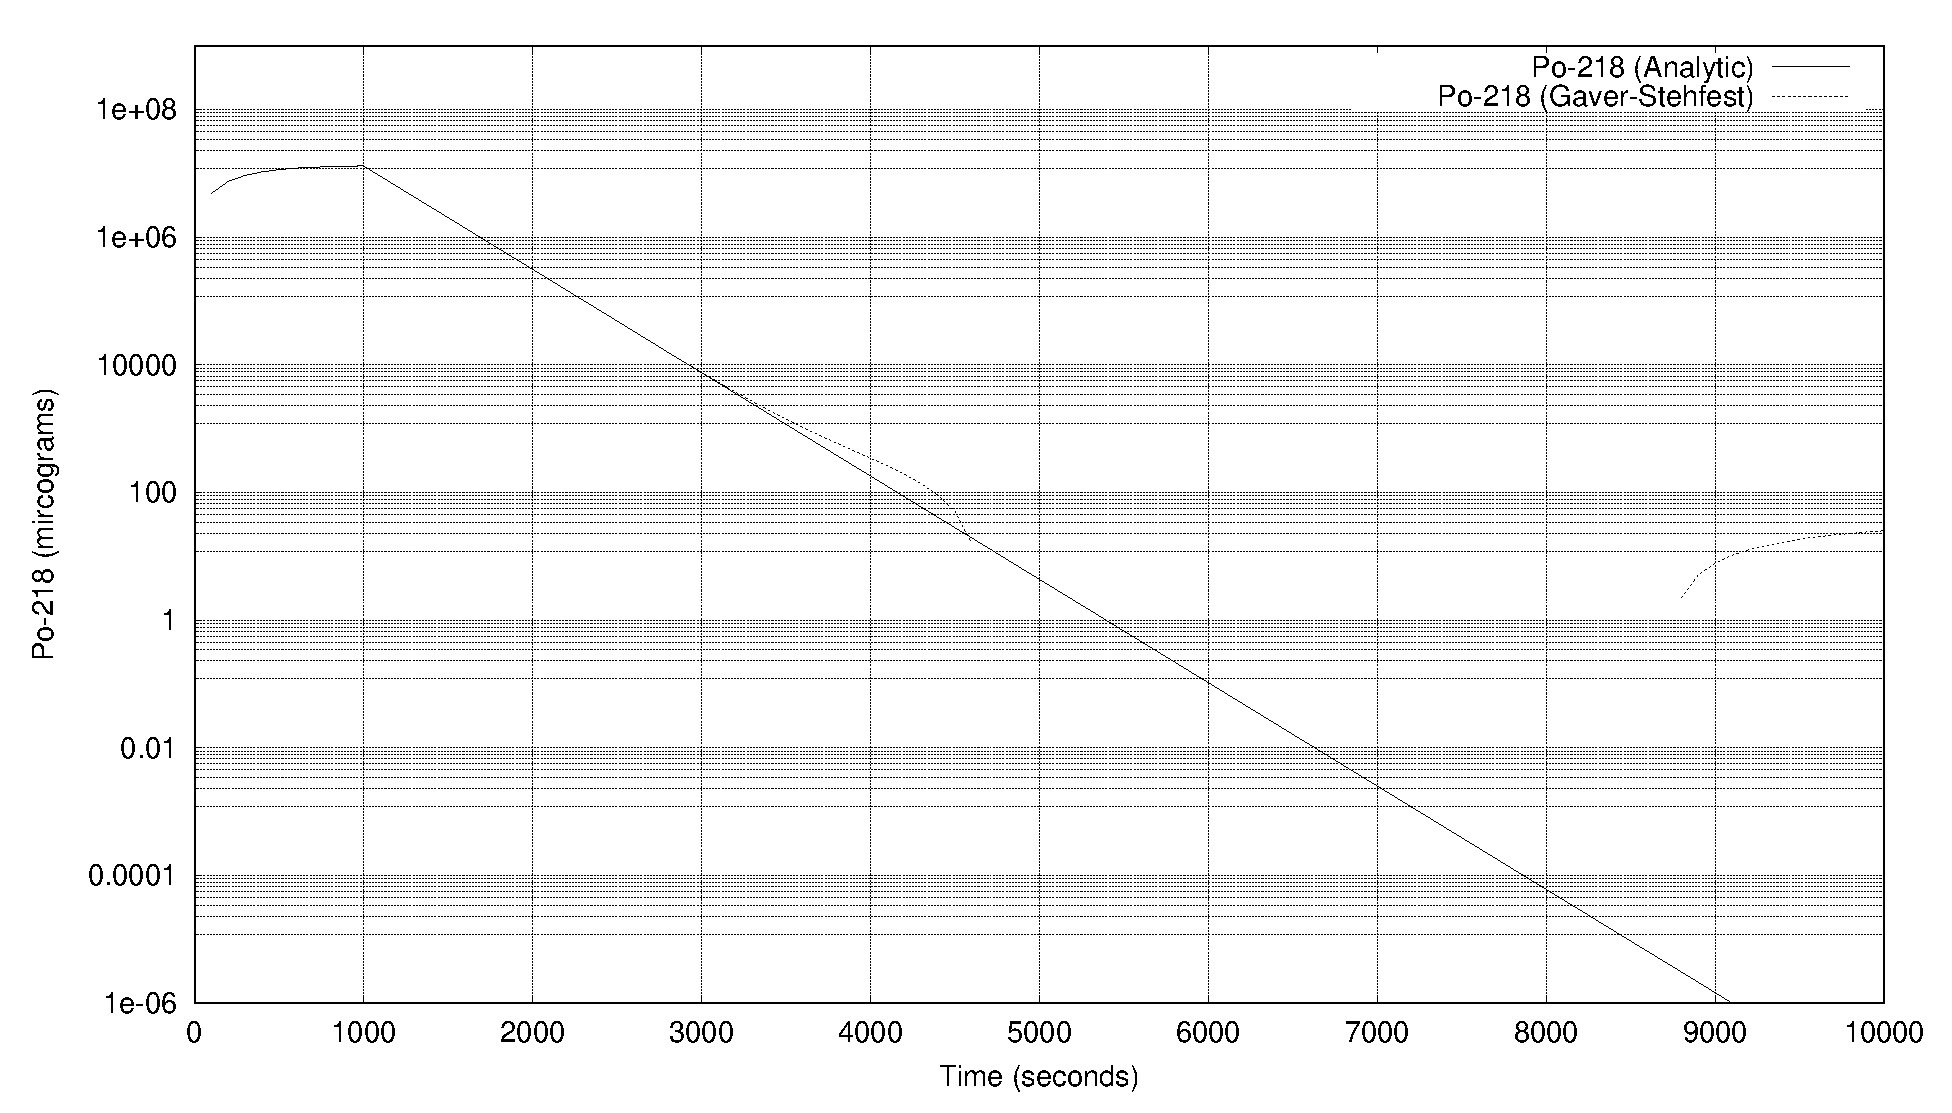
\includegraphics[width=15.0cm]{chapters/methodology_activity/plots/po-218/po218_po218.eps}
		\captionsetup{font={it}}
		\caption{Decay of Po-218: Analytic and Gaver-Stehfest Calculations \cite{jeff311}}
		\label{fig:po218decay}
	\end{center}
\end{figure}

The numeric solution only requires the equation to be solved in the s-domain; the Gaver-Stehfest algorithm performs the inversion.  It is worth the extra effort to derive and implement an analytic solution, as the numeric is only an approximation.  Examples of the pitfalls of the numeric solution are that it can give negative amounts of an isotope and the difference between the numeric and analytic calculated amounts can become quite large when the isotope decays away to a very small value.  Figure \ref{fig:po218decay} shows the predicted decay of a sample of Po-218 irradiated for 1,000s, and sampled until 10,000s.  In the region between 4,000s and 9,000s the amount from the numeric calculation drops below zero, whereas the analytic calculation remains above zero, as would be expected.



\section{Computational Methods}

\subsection{Activity V1}

The Activity V1 program has been developed in Fortran and takes advantage of MPI (Message Parsing Interface) to speed up calculation times by allowing the use of multiple processes in parallel.  It has a self contained maths library, although this could be improved in the future by using optimised maths libraries for certain functions (e.g. linear algebra).

The code was developed on a Debian based distribution of Linux, but it should be supported on other variants of Linux and Unix, and does not require any specialist hardware.

\begin{figure}[!h]
	\centering
	\begin{tikzpicture}[node distance=2cm]
	% Row 1
	\node (1a) [process] {\makecell[l]{User input file\\read into memory}};
	\node (1b) [process, right of=1a, xshift=2.5cm] {\makecell[l]{Load cross section\\data for isotopes\\(specified by user)}};
	\node (1c) [process, right of=1b, xshift=2.5cm] {\makecell[l]{Load ion exyz\\trajectory file}};
	% Row 2
	\node (2a) [process, below of=1a] {\makecell[l]{Loop through time steps:\\calculate amount/activity\\of each isotope}};
	\node (2b) [process, right of=2a, xshift=2.5cm] {\makecell[l]{Split polynomial fit\\into segments: calculate\\all possible reaction rates}};
	\node (2c) [process, right of=2b, xshift=2.5cm] {\makecell[l]{Use MPI: Fit polynomial\\to trajectory of each ion\\and take superposition}};
	% Row 3
	\node (3a) [process, below of=2a] {\makecell[l]{Output data and\\charts to user}};
	
	% arrows
	\draw [thick,->] (1a) -- (1b);
	\draw [thick,->] (1b) -- (1c);
	\draw [thick,->] (1c) -- (2c);
	\draw [thick,->] (2c) -- (2b);
	\draw [thick,->] (2b) -- (2a);
	\draw [thick,->] (2a) -- (3a);
	%\draw [->] (isotope1) -- (isotope2);
	%\draw [->] (isotope2) -- (stable);
	\end{tikzpicture}
	\captionsetup{font={it}}
	\caption{Flow chart of major processes in the Activity code}
	\label{fig:processflowchart}
\end{figure}

The user is required to prepare an input file that contains the instructions required to perform a calculation.  In addition to the input file, the user must provide an \acrshort{exyz} ion trajectory file output by \acrshort{srim}.  Activity will read in the user input file, and the \acrshort{srim} and data files listed within, before performing the calculation.  Figure \ref{fig:processflowchart} shows a flowchart of the major steps the code performs.

There are various settings in the user input file, but the main ones relating to the simulated experiment are:

\begin{itemize}
	\item Element composition of target (percentage by mass).
	\item Beam flux (current), energy, duration and area on target.
	\item Activity measurement time (end of the ``experiment").
	\item Material density.
	\item Target thickness.
\end{itemize}

A brief manual that accompanies the program is in the appendix section \ref{section:activityv1manual} and the published paper that accompanies the code is in section \ref{section:activityv1published}.  The cross section data is taken from the existing TENDL-2013 datafile.



\subsection{Activity V2}

A second program was developed to use Python rather than Fortran.  One problem that motivated this was occasionally a particular isotope would cause the code to crash, and a second issue was the complication of compiling the code for new users.  The Python version runs with relatively few interventions by the user and it handles errors in the data more gracefully than the Fortran version.  The procedure it follows is similar to the Activity V1 code and the manual is included in appendix section \ref{section:activityv2manual}.

Due to a variation in range of energies in cross section data files, the cross section data was computed from scratch using the TALYS code and the BlueBEAR HPC.


\FloatBarrier
\subsection{Ion Trajectory Data}

The \acrshort{srim} code is used to generate ion trajectory data.  This uses a quantum mechanical treatment of ion-atom collisions and statistical algorithms to speed up the process\cite{srimwebsite}.

\begin{figure}[htp]
  \begin{center}
    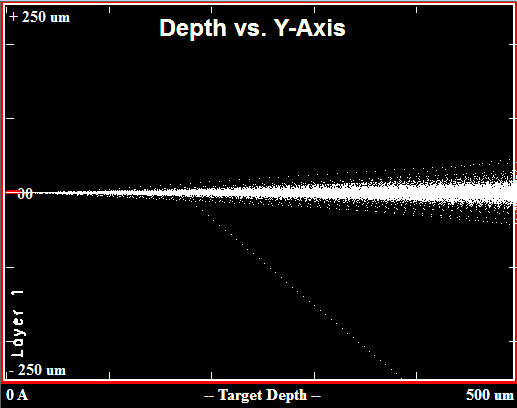
\includegraphics[scale=0.55]{chapters/methodology_activity/images/ion_transport.png}
    \caption{36MeV Ion Track}
    \label{graph:graph1}
  \end{center}
\end{figure}

The trajectory data files used by both versions of the Activity code will be created using \acrshort{srim} for the required beam energy and target combinations.

\begin{figure}[htp]
  \begin{center}
    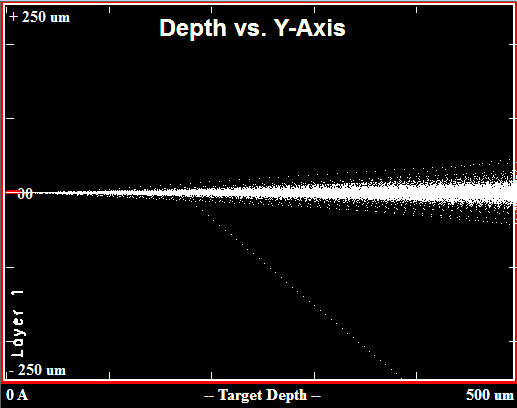
\includegraphics[scale=0.55]{chapters/methodology_activity/images/ion_transport.png}
    \caption{36MeV Ion Track}
    \label{graph:graph1}
  \end{center}
\end{figure}

The target is set as pure Iron, and due to the way \acrshort{srim} functions, the structure type is inconsequential.  At just 0.5mm in thickness, the 36MeV ions pass through the targets and exit with an energy above 30MeV, and the exyz.txt data file covers this range of ion energies.


\subsection{Activity Code Assumptions}

A number of assumptions have been made for both codes to simplify the model.  These may be addressed in future versions if development of the code continues.  The flux of the beam is assumed to be constant at any depth into the material.  Charged particle irradiation is ignored completely from the decay of radioactive isotopes in the target, and the amount of beta radiation may determine how the target is handled.

Gammas are assumed to be emitted isotropically and degrade only due to the increase in surface area as the distance from the source increases.  No consideration is given to the dispersion of radioactive isotopes through the target material, how much material the gammas must pass through or how much air they must go through in order to reach the person (or measuring device).

These assumptions and possible improvements are considered in chapter \ref{chapter:futurework}.


\FloatBarrier



\subsection{Foil Activation by Neutron Irradiation}

%\subsection{Introduction}

An additional feature was added to the Activity V2 code to estimate neutron activity based on the existing code developed to calculated ion activation.  It is a simple non-transport neutron activation code, used to estimate the activity and subsequent cooling of materials irradiated by neutrons.  A single energy neutron flux or Maxwell-Boltzmann distribution may be selected by the user and the TALYS generated database is used to provide cross sections for calculating reaction rates.  Finally, the previously derived extended Bateman equations are used to calculate isotopes at time t after irradiation begins.








\section{Cyclotron Irradiated Iron}

\subsection{Cyclotron Beam Line}

The Scanditronix MC40 cyclotron at the University of Birmingham has several beamlines and is capable of accelerating protons, deuterons, Helium 3 and Helium 4 with fluxes and energy ranges detailed in table \ref{table:scanditronixlimits}.  After running a simulation with \acrshort{srim}, the 36MeV protons were expected to create an average of 15.8 vacancies each.

\begin{table}[h]
\begin{center}
\begin{tabular}{c c c c}
\hline\hline
Particle & Energy (MeV) & Max Current (micro A) & Flux (ions per second)\\
\hline\hline
p & 8-40 & 60 & $3.75 \times 10^14$ \\
d & 8-40 & 30 & $1.87 \times 10^14$ \\
${}^4 He^{2+}$ & 8-53 & 30 & $9.36 \times 10^13$ \\
${}^3 He^{2+}$ & 4-20 & 60 & $1.87 \times 10^14$ \\
\hline\hline
\end{tabular}
\end{center}
\caption{Beam Characteristics of the Scanditronix MC-40}
\label{table:scanditronixlimits}
\end{table}

The cyclotron is located in one room, and several beam lines run from the cyclotron to other rooms in the cyclotron building.  The operation room is separate from the cyclotron and beam line rooms (figure \ref{fig:cyclotronlayout}).

\begin{figure}[htp]
  \begin{center}
    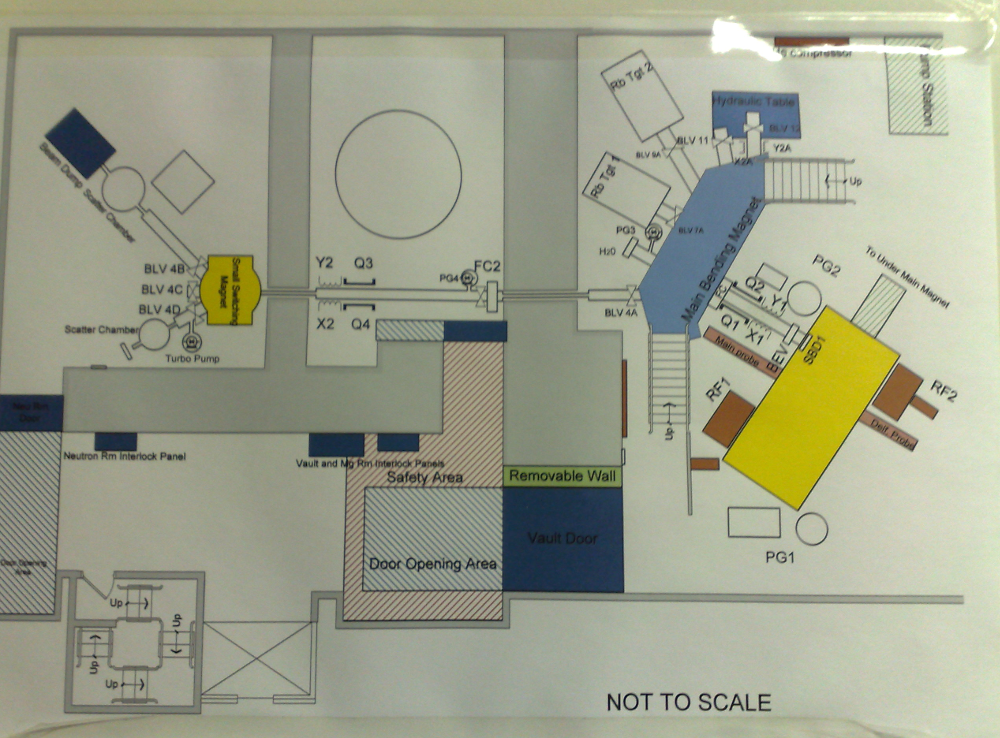
\includegraphics[scale=0.7]{chapters/methodology_activity/images/cyclotron_layout.png}
    \caption{Cyclotron layout - main hall and beam lines}
    \label{fig:cyclotronlayout}
  \end{center}
\end{figure}

The iron sample was held perpendicular to the beam line, with the ions passing through the 0.5mm thickness of the sheet.  The beam area was approximately $6.4 \times 10^{-5} m^2$, irradiating a volume of approximately $3.2 \times 10^{-8} m^3$.  The target was irradiated for 300 seconds at 0.5 micro amps and it was expected to cause over $1.4 \times 10^{16}$ displacements within the volume of iron targetted by the beam.  With a number density of approximately $8\times10^{28}$ atoms per cubic meter, giving a relatively low damage dose, when compared to that expected over the lifetime of a component within the reactor, of $5 \time 10^{-6}$ \acrshort{dpa}.

\begin{figure}[htp]
  \begin{center}
    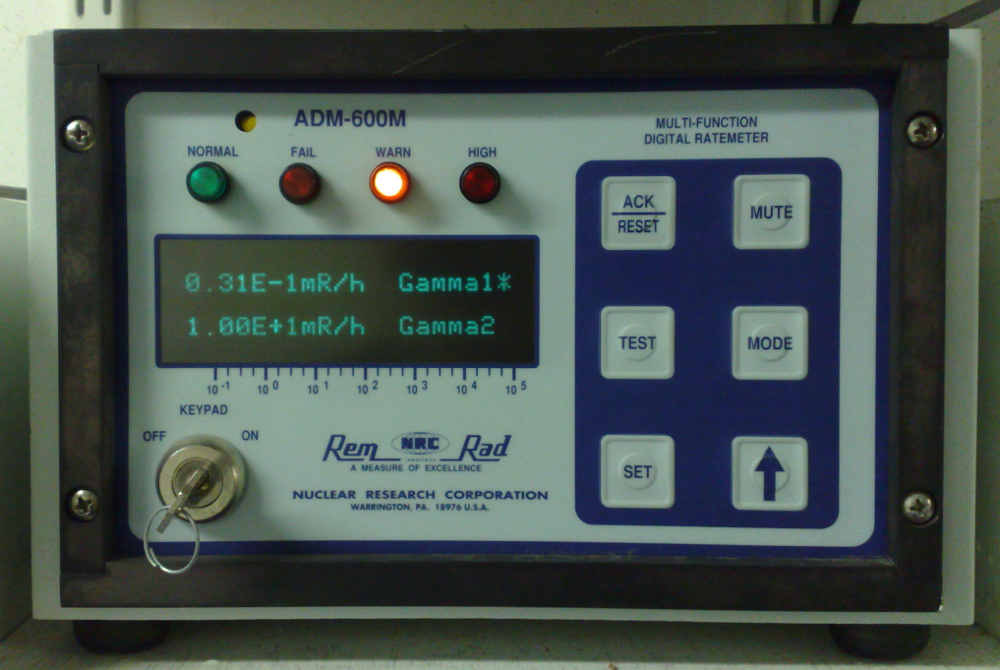
\includegraphics[scale=0.7]{chapters/methodology_activity/images/gamma_warning.png}
    \caption{Gamma warning alarm during 0.5 microamp 36MeV proton irradiation of iron }
    \label{fig:gammawarning}
  \end{center}
\end{figure}

During irradiation, the amount of gamma radiation released was enough to trip the alarm for the room (figure \ref{fig:gammawarning}).  The proton fluence was less than 1\% of the maximum fluence capable of being produced by the cyclotron, so this was definitely a concern.  To increase the damage dose, and keep to a shorter period of time, the current would most probably be increased to a much higher percentage, also increasing the rate of Gammas produced during irradiation.


\subsection{Measurement of Sample Activity}

The sample was too radioactive to safely handle immediately after irradiation, so it was left to cool for several days before taking measurements.  After it had cooled, a high purity germanium detector (figure \ref{fig:hpge}) was used to measure the activity of the irradiated sample.

\begin{figure}[htp]
  \begin{center}
    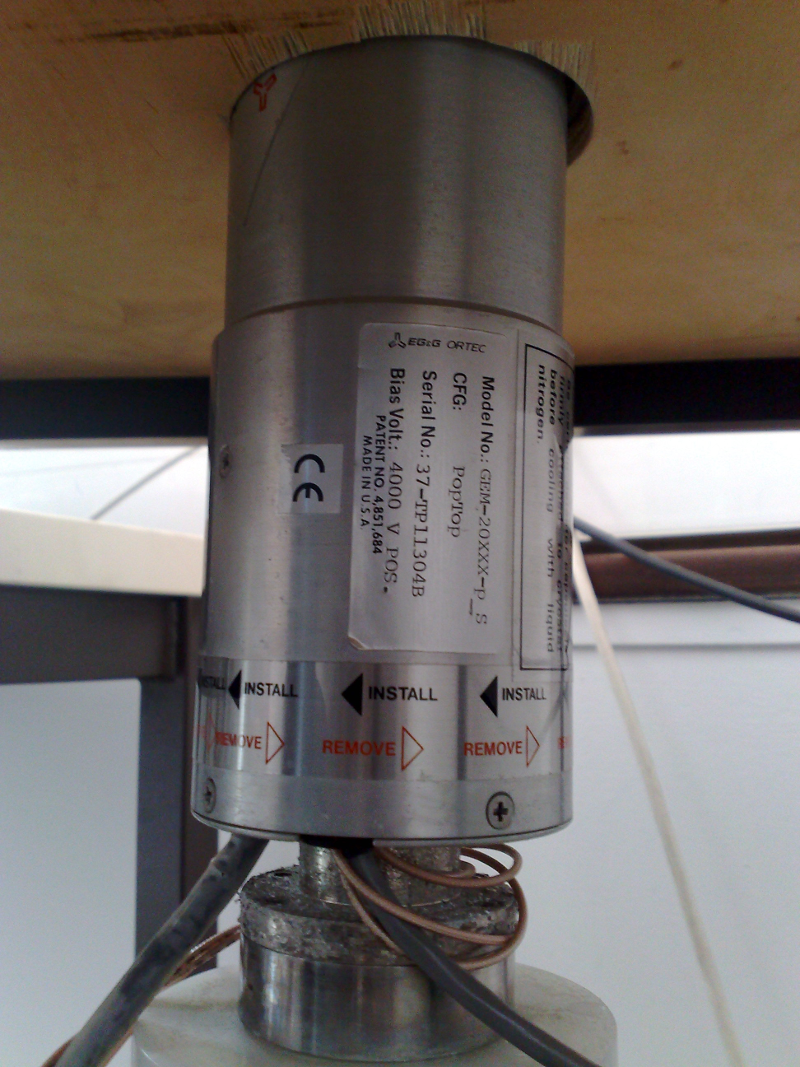
\includegraphics[scale=0.8]{chapters/methodology_activity/images/hpge.png}
    \caption{High Purity Germanium Detector}
    \label{fig:hpge}
  \end{center}
\end{figure}

The detector and preamplifier are both cooled by liquid nitrogen to 77K, as the band-gap of germanium is 0.7eV and the thermal motion of electrons and nuclei at higher temperatures would induce currents causing noise and interference in the detector.  As a gamma ray enters the detector it creates an electron-hole pair in the medium of the detector.  The holes and electrons are attracted to the center and to the outer cylinder of the detector, or vice versa.



\subsection{Prediction of Activity}

Following the measurement of the thin target, in the first instance the predicted activity will be estimated using the average ion energy, the cross section of this energy and the two reactions that result in Co-55 (${}^{54}_{26} Fe (p, \gamma) {}^{55}_{27} Co$ and ${}^{56}_{26} Fe (p, 2n) {}^{55}_{27} Co$).  The activity code (version 1 and version 2) are then used to predict the activity of the sample as well as the expected gamma spectra.


